

\section{Auswertung}
\subsection{Überprüfung der Bragg Bedingung}
Der fest eingestellte Kristallwinkel liegt bei
\begin{equation*}
  \theta = 14°
\end{equation*}
\begin{figure}
  \centering
  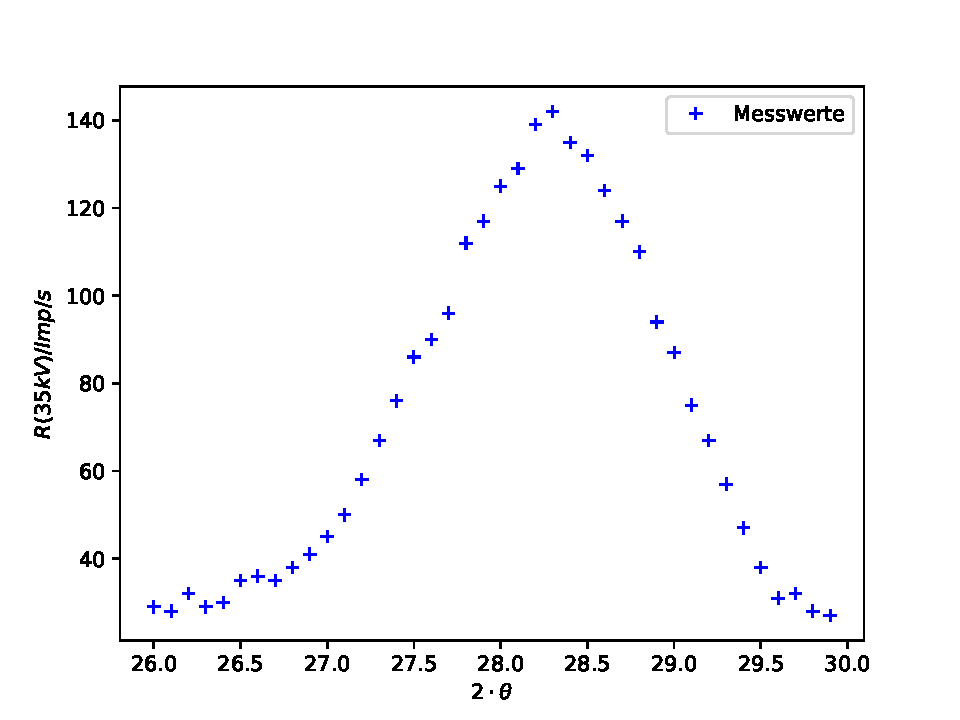
\includegraphics[width=\textwidth]{bragg.pdf}
  \caption{Die Intensität der Röntgenstrahlen}
  \label{fig:bragg}
\end{figure}
In Abbildung \ref{fig:bragg} sind die gemessenen Werte aufgetragen.
Aus diesen Werten ergibt sich das Maximum bei
\begin{equation}
  \theta = 14,15°
\end{equation}
Der Winkel weicht um $\Delta\theta = 0,15°$ ab,
sodass die Bragg Bedingung erfüllt ist.
Das entspricht einer prozentualen Abweichung zum Sollwinkel von 1,07\%.

\subsection{Das Emissionsspektrum einer Cu-Röntgenröhre}
\begin{figure}[H]
  \centering
  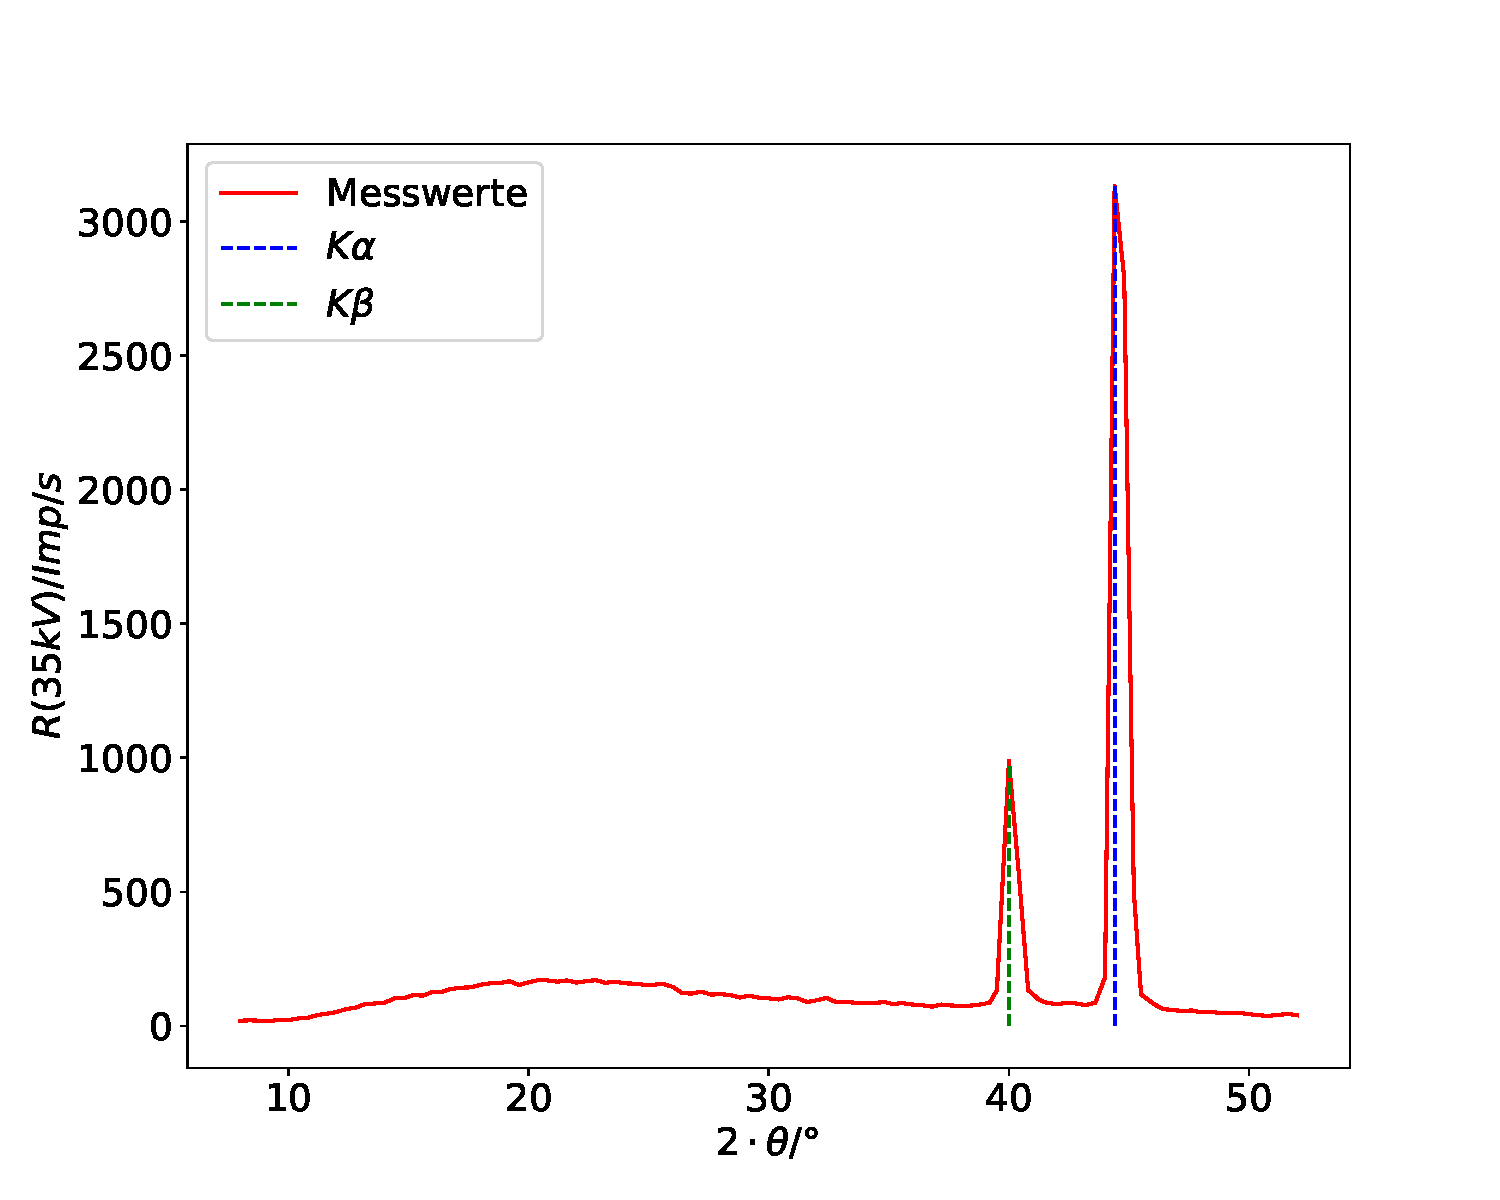
\includegraphics[width=\textwidth]{cu2.pdf}
  \caption{Röntgenspektrum der Cu-Röntgenröhre}
  \label{fig:cu}
\end{figure}
In Abbildung \ref{fig:cu} sind die $K_{\alpha}-, K_{\beta}-$Linien,
sowie der Bremsberg zu sehen.
Der Bremsberg geht von $2\theta =$10° bis ca 40°.
Der Grenzwinkel wird aus den Messwerten entnommen und beträgt $\theta = 5°\pm 0,1°$.
Daraus ergibt sich mit Formel (\ref{eqn:bragg})
\begin{equation*}
  \lambda_{min}= (35,106\pm 0,703) \, \mathrm{pm}
\end{equation*}
Mit Formel (\ref{eqn:E}) ergibt sich die Maximale Energie zu
\begin{equation*}
  E_{max} = (35,3 \pm 0,7)\, \mathrm{keV}
\end{equation*}
Die Energie hat somit eine prozentuale Abweichung von 0,91\%
zum theoretischen Wert von $35\, \mathrm{keV}$

Mithilfe der Messwerte werden nun die Halbwertsbreiten bestimmt.
Diese sind in den Abbildungen \ref{fig:h1} und \ref{fig:h2} dargestellt.
\begin{figure}[H]
  \centering
  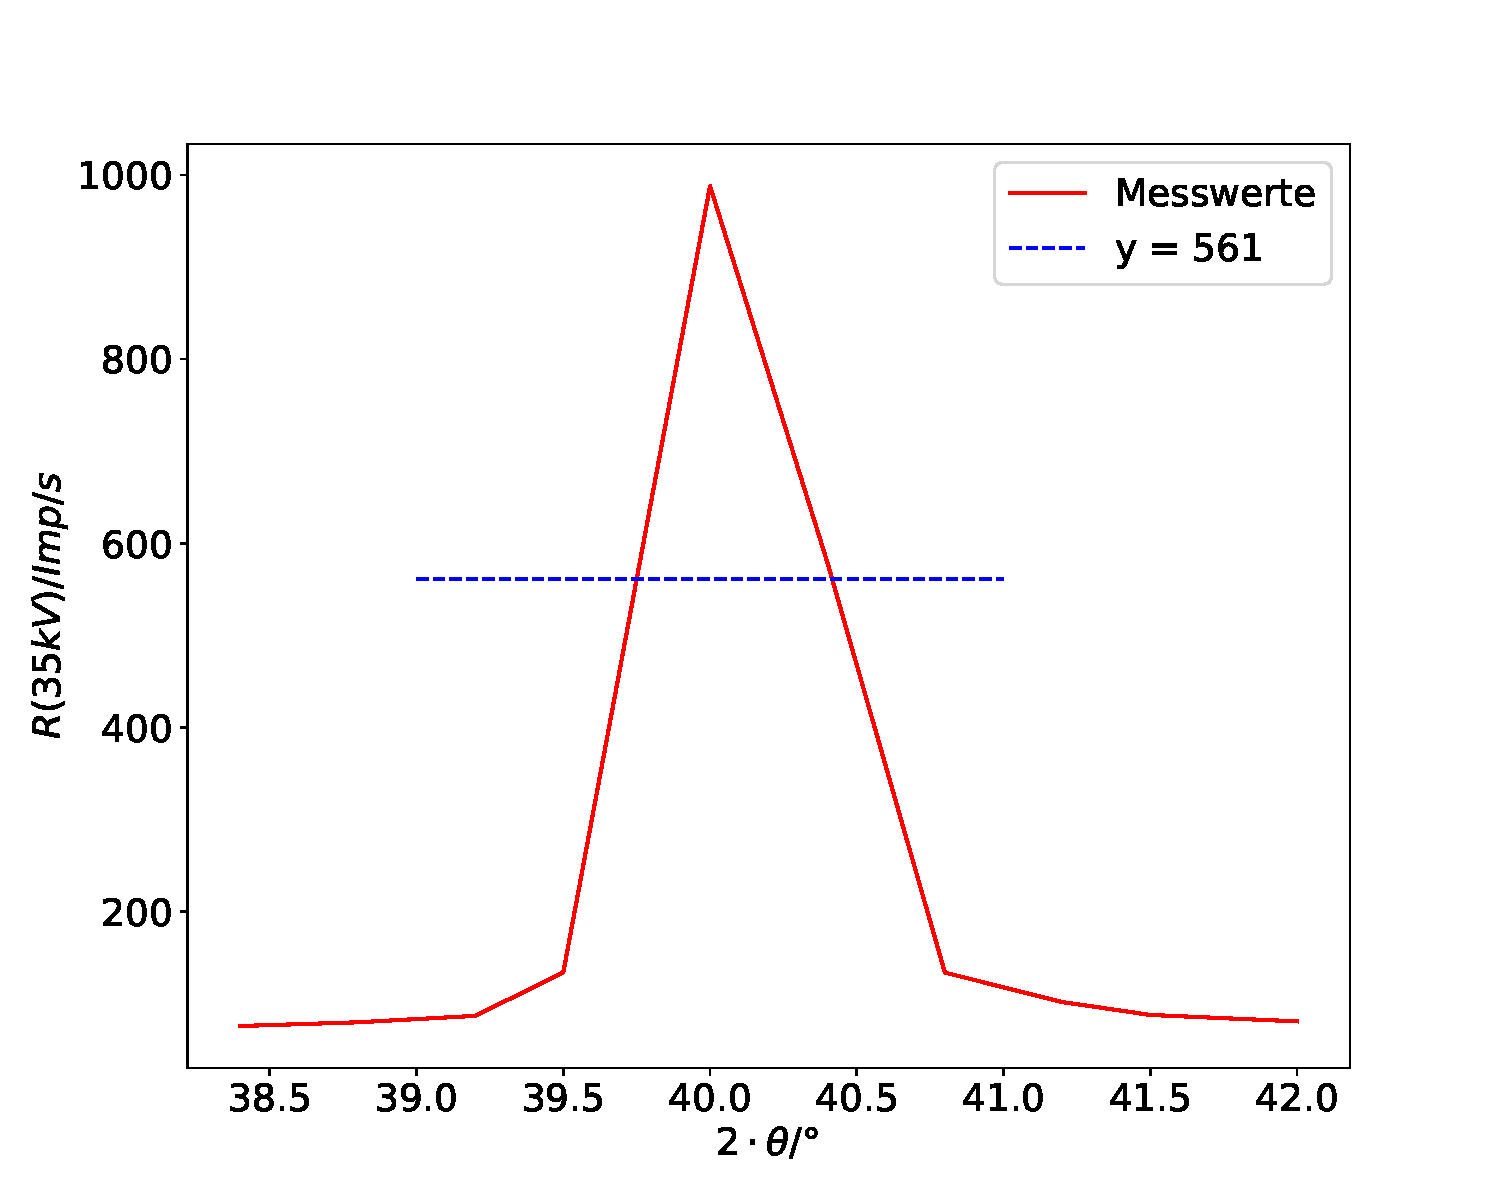
\includegraphics[width=\textwidth]{halbwerts1.pdf}
  \caption{Halbwersbreite von $K_{\beta}-Peaks$}
  \label{fig:h1}
\end{figure}
\begin{figure}[H]
  \centering
  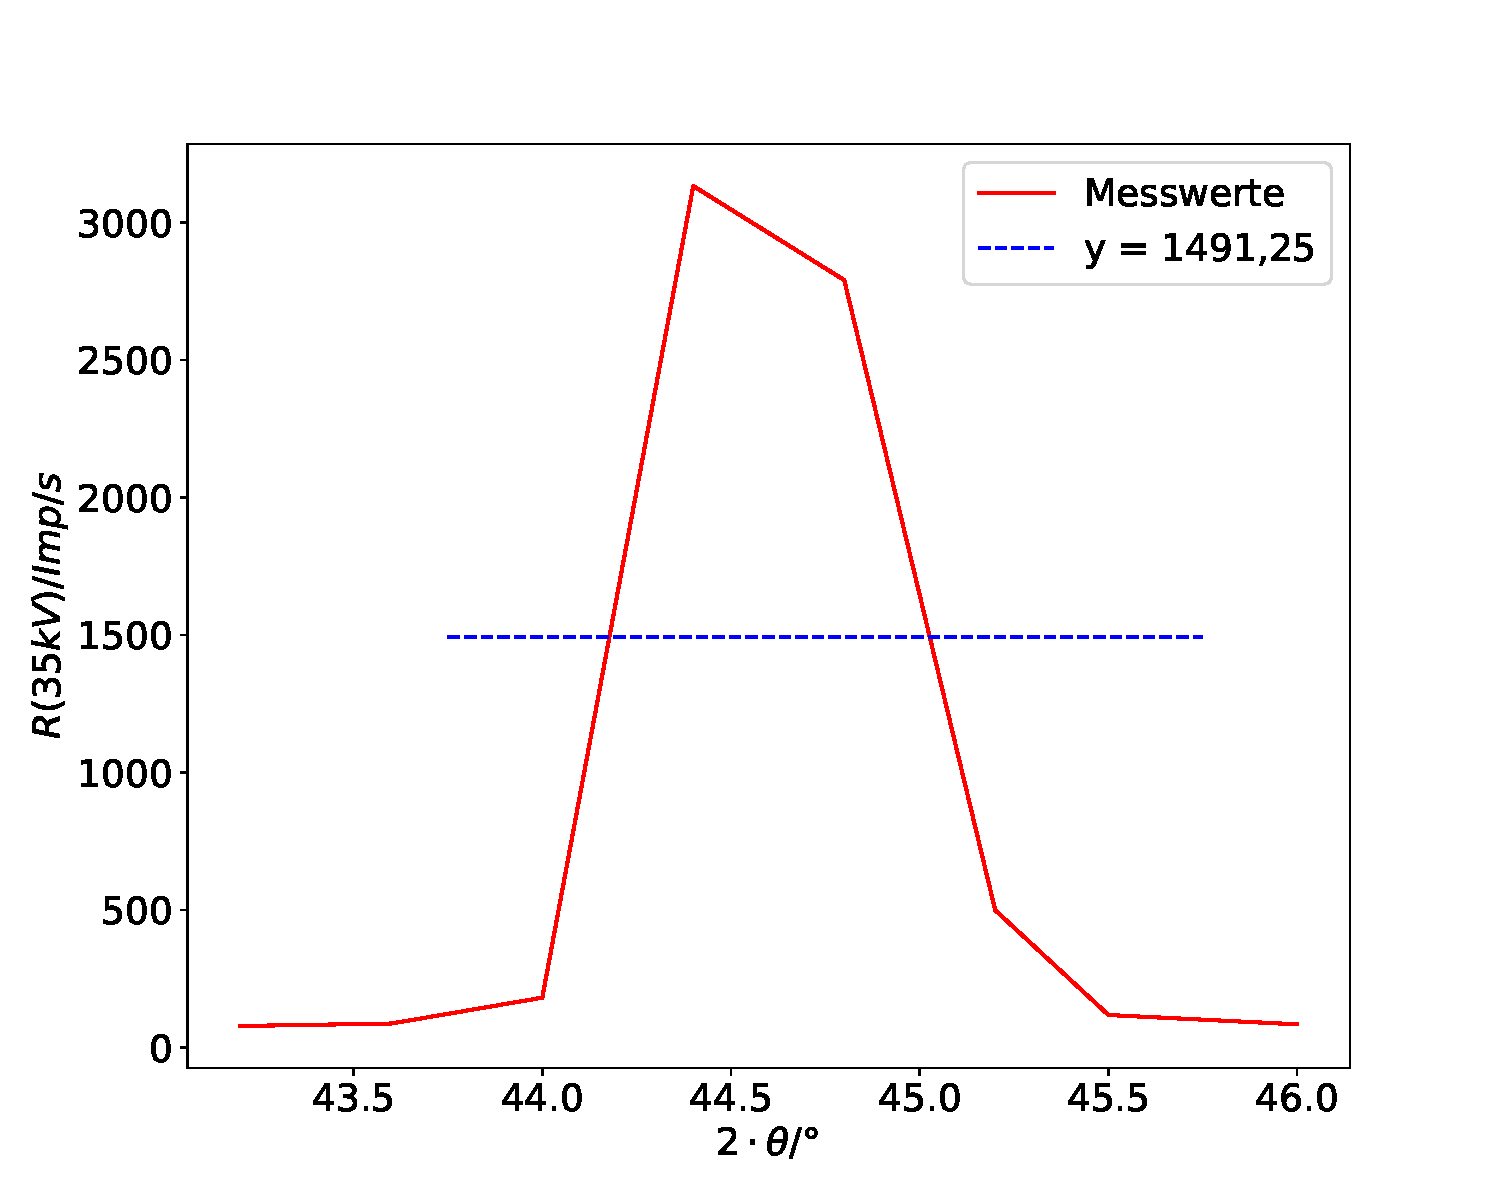
\includegraphics[width=\textwidth]{halbwerts2.pdf}
  \caption{Halbwertsbreite von $K_{\alpha}-Peaks$}
  \label{fig:h2}
\end{figure}
Das Auflösungsvermögen berechnet sich mit der Formel
\begin{equation*}
  U = \frac{E}{\Delta E}
\end{equation*}
Die Ergebnisse sind in Tabelle \ref{tab:aufl} dargestellt.
\begin{table}
  \centering
  \caption{Auflösungsvermögen}
  \label{tab:aufl}
  \begin{tabular}{c c c c c c c}
    \toprule {} & {$\theta_L$/ °} & {$E_L$/ keV} & {$\theta_R$/ °} & {$E_R$/ keV} & {$\Delta E$/ keV} & {U}\\
    \midrule
$K_{\alpha}$ & 44\pm 0,1 & 4,431\pm0,008  & 45,5\pm 0,1 & 4,316\pm0,007  & 0,084\pm0,001 & 51,86\pm0,63 \\
$K_{\beta}$ & 39,5\pm 0,1 & 4,839\pm0,010 & 40,75\pm 0,1 & 4,715\pm 0,010 & 0,124 & 38,52\pm0,08\\
\bottomrule
\end{tabular}
\end{table}
\\

Die entnommenen Winkel für $K_{\beta}$ und $K_{\alpha}$ lauten:
\begin{align*}
  \theta_{K_{\alpha}} &= 22,2°\\
  \theta_{K_{\beta}} &= 20°
\end{align*}
Die bestimmten Wellenlängen und Energien werden
mit den Formeln (\ref{eqn:bragg}) und
\begin{equation}
  E = h\cdot \frac{c}{\lambda}
  \label{eqn:E}
\end{equation}
 bestimmt.

\begin{align*}
  \lambda_{K_{\alpha}} &= 152,194 \, \mathrm{pm} & \lambda_{K_{\beta}} &= 137,766\, \mathrm{pm} \\
  E_{K_{\alpha, berechnet}} &= 8,146\, \mathrm{keV} &  E_{K_{\beta, berechnet}} &= 8,999\, \mathrm{keV} \\
  E_{K_{\alpha, theoretisch}} &= 8,048\, \mathrm{keV} & E_{K_{\beta, theoretisch}} &= 8,906\, \mathrm{keV} %\cite{wert}
\end{align*}
Die theoretisch zu erwartenden Werte wurden \cite{wert} entnommen.
Die prozentualen Abweichungen ergeben sich zu
\begin{align}
  \Delta E_{K_{\alpha}} &= 1,22\%\\
  \Delta E_{K_{\beta}} &= 1,04\%
\end{align}
Mit den Formeln
\begin{align}
  E_{abs}&= R_{\infty}(z-\sigma_1)^2\\
  E_{k_\alpha} &= R_{\infty}(z-\sigma_1)^2-R_{\infty}\frac{1}{4}(z-\sigma_2)^2\\
  E_{k_\beta} &= R_{\infty}(z-\sigma_1)^2-R_{\infty}\frac{1}{9}(z-\sigma_3)^2\
\end{align}
ergeben sich nun die Abschirmkonstanten $\sigma_1$, $\sigma_2$ und $\sigma_3$.
$E_{abs}$ ist hierbei 8980\,eV,
z ist die Ordnungszahl von Kupfer und hat einen Wert von 29.\cite{Z}
$R_{\infty}$ ist die Rydbergenergie mit einem Wert von $13,6\, \mathrm{eV}$.\cite{Anleitung}
\begin{align}
  \sigma_1 &= 3,303\\
  \sigma_2 &= 26,555\\
  \sigma_3 &= 29,081
\end{align}




%Die Abschirmkonstante $\sigma_K$ berechnet sich nun mit der Formel
%\begin{align*}
%  \sigma_K &= Z-\sqrt{\frac{-4\cdot (E_{K_{\alpha}}- E_{K_{\beta}})}{R_\infty}}\\
%  \sigma_K &= 13,161
%\end{align*}
%Z ist die Ordnungszahl von Kupfer und hat einen Wert von 29.\cite{Z}
%$R_{\infty}$ ist die Rydbergenergie mit einem Wert von $13,6\, \mathrm{eV}$.\cite{Anleitung}


\subsection{Das Absorptionsspektrum}
Die Winkwl der K-Kanten von Brom, Strontium und Zirkonium werden aus den Messwerten entnommen,
bzw. aus den Abbildungen \ref{fig:brom}, \ref{fig:strontium} und \ref{fig:zirkonium} entnommen.
\begin{align*}
\theta_{Brom} &= 13,05°\\
\theta_{Strontium} &= 10,85°\\
\theta_{Zirkonium} &= 9,75°
\end{align*}
Mit den Formeln \ref{eqn:bragg} und \ref{eqn:E} werden zunächst die einzelnen Wellenlängen
und dann die Energien bestimmt.
Diese sind in Tabelle \ref{tab:alamde} aufgelistet.

\begin{table}
  \centering
  \caption{Wellenlängen und Energien}
  \label{tab:alamde}
  \begin{tabular}{c c c}
    \toprule {} & {Wellenlänge / pm} & {Energie/ keV}\\
    \midrule
Brom      & 90,95 & 13,632 \\
Strontium & 75,82 & 16,352 \\
Zirkonium & 68,21 & 18,176 \\
\bottomrule
\end{tabular}
\end{table}

\begin{figure}
  \centering
  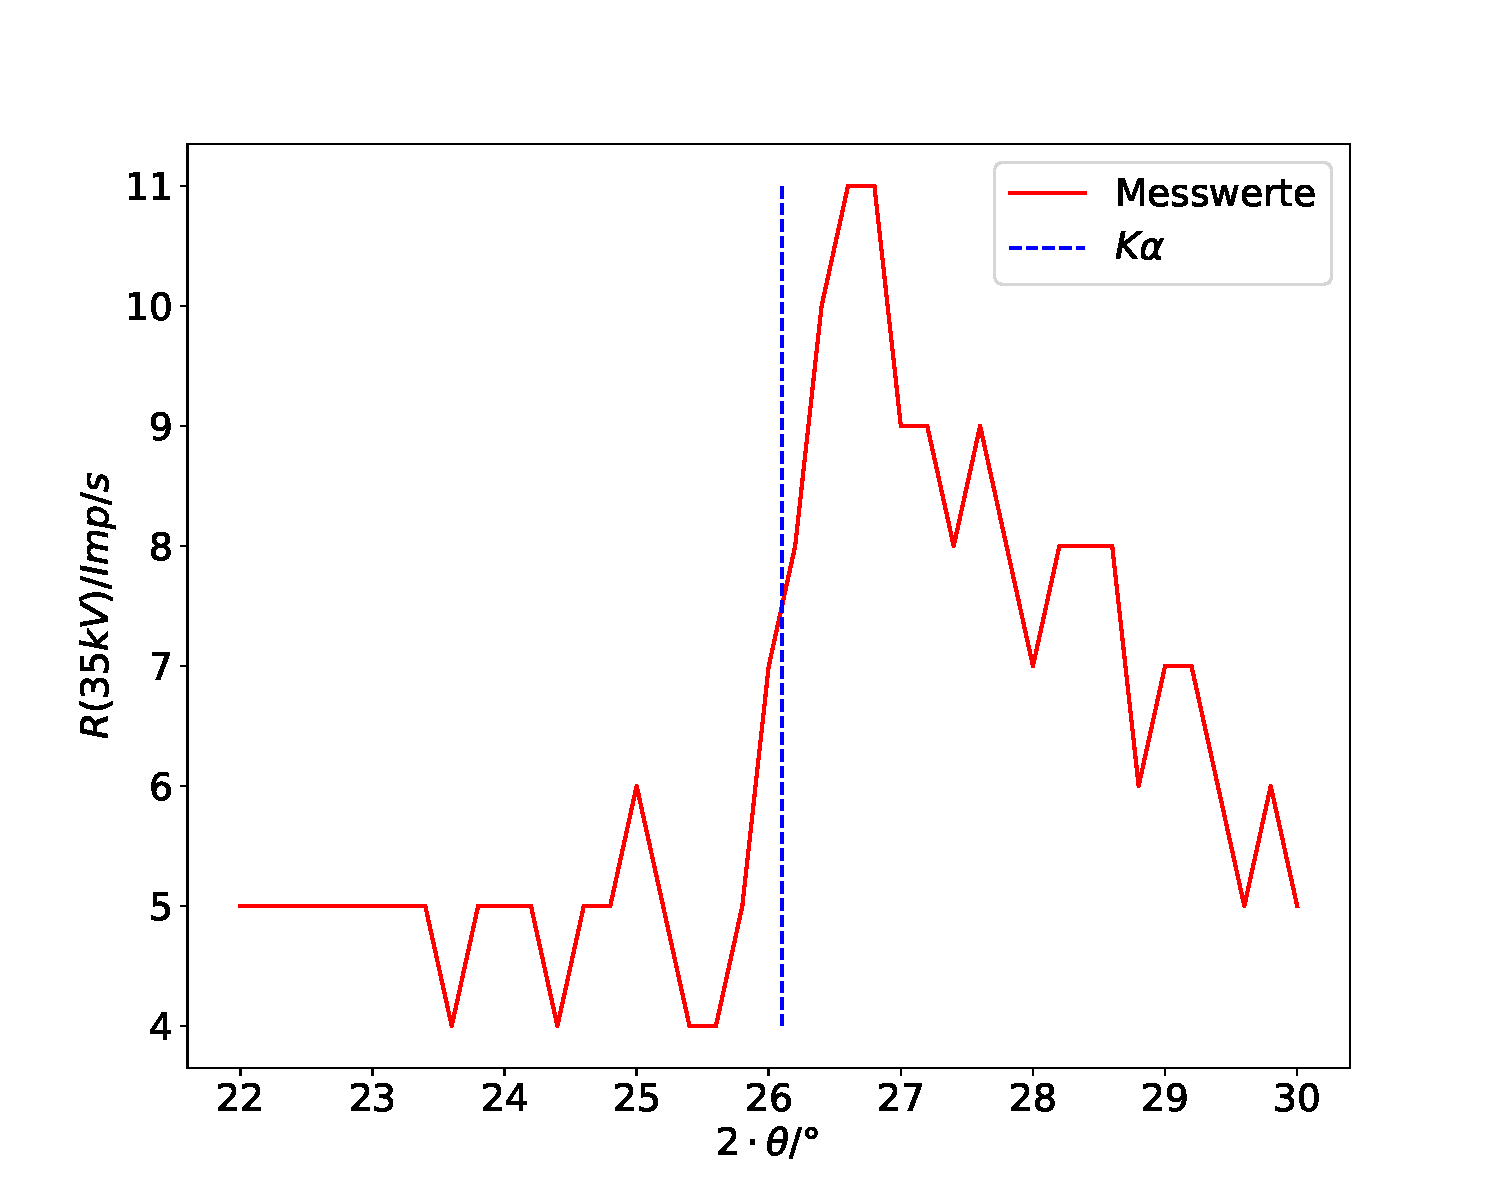
\includegraphics[width=\textwidth]{brom.pdf}
  \caption{Absorptionsspektrum von Brom}
  \label{fig:brom}
\end{figure}
\begin{figure}
  \centering
  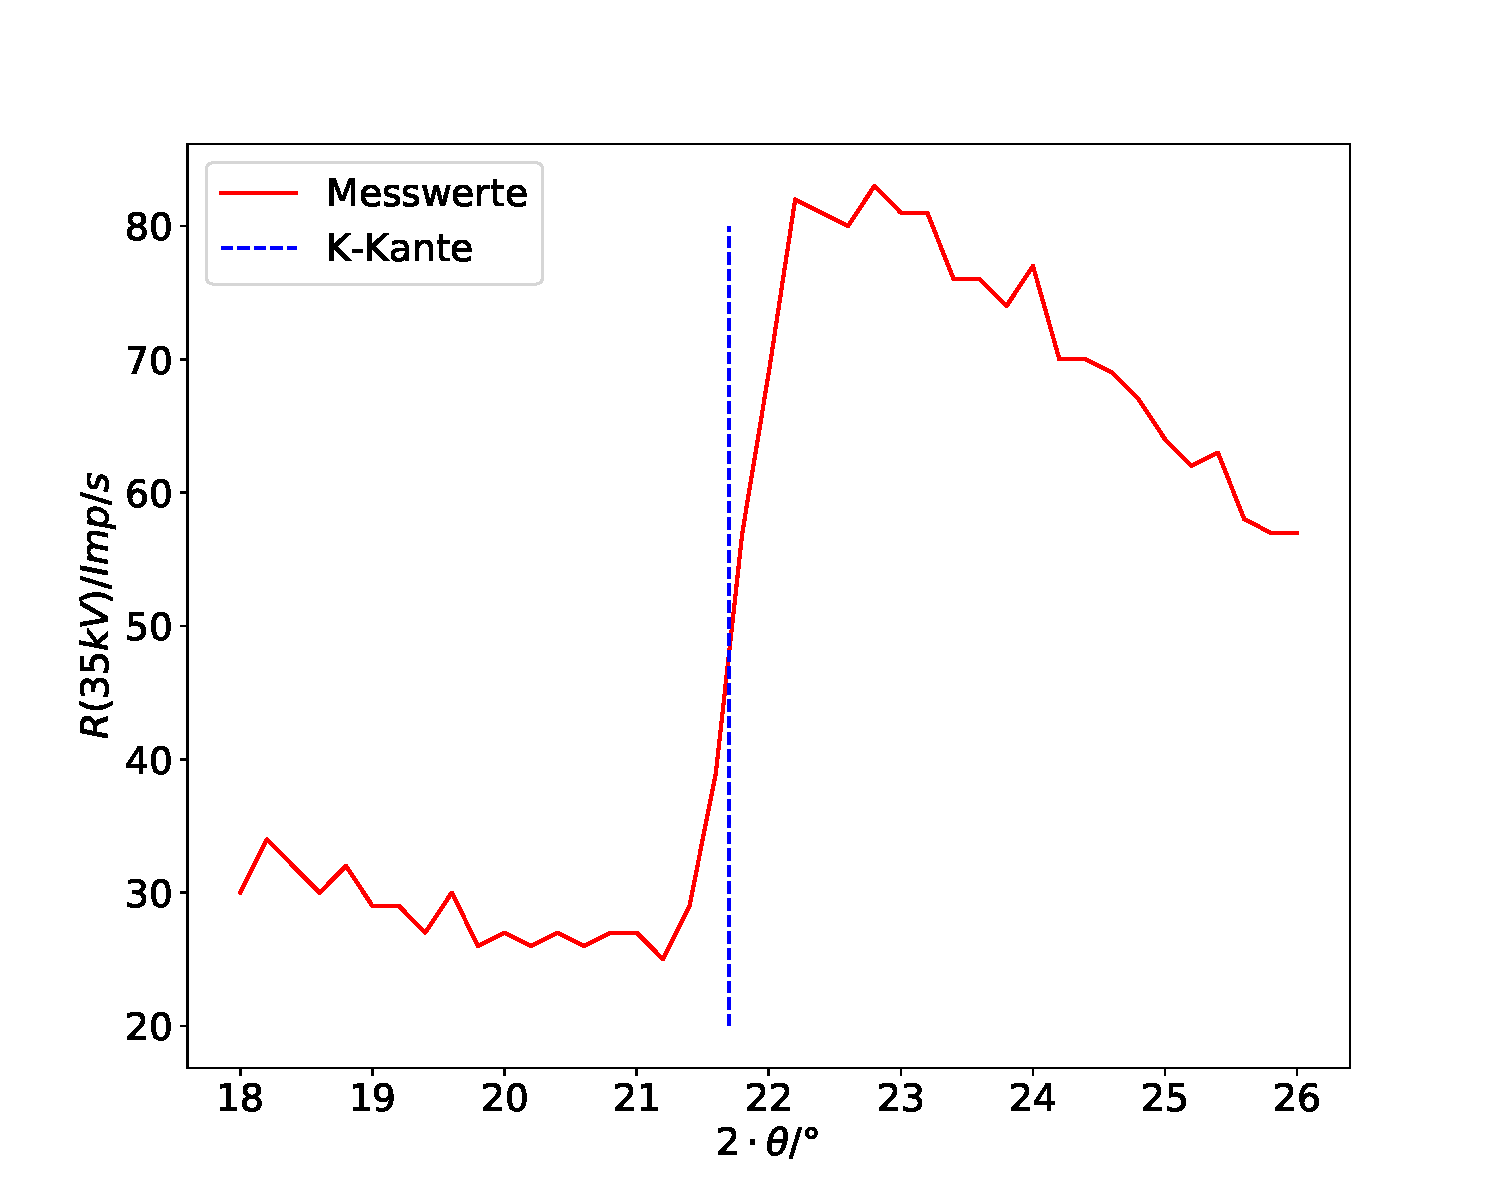
\includegraphics[width=\textwidth]{strontium.pdf}
  \caption{Absorptionsspektrum von Strontium}
  \label{fig:strontium}
\end{figure}
\begin{figure}
  \centering
  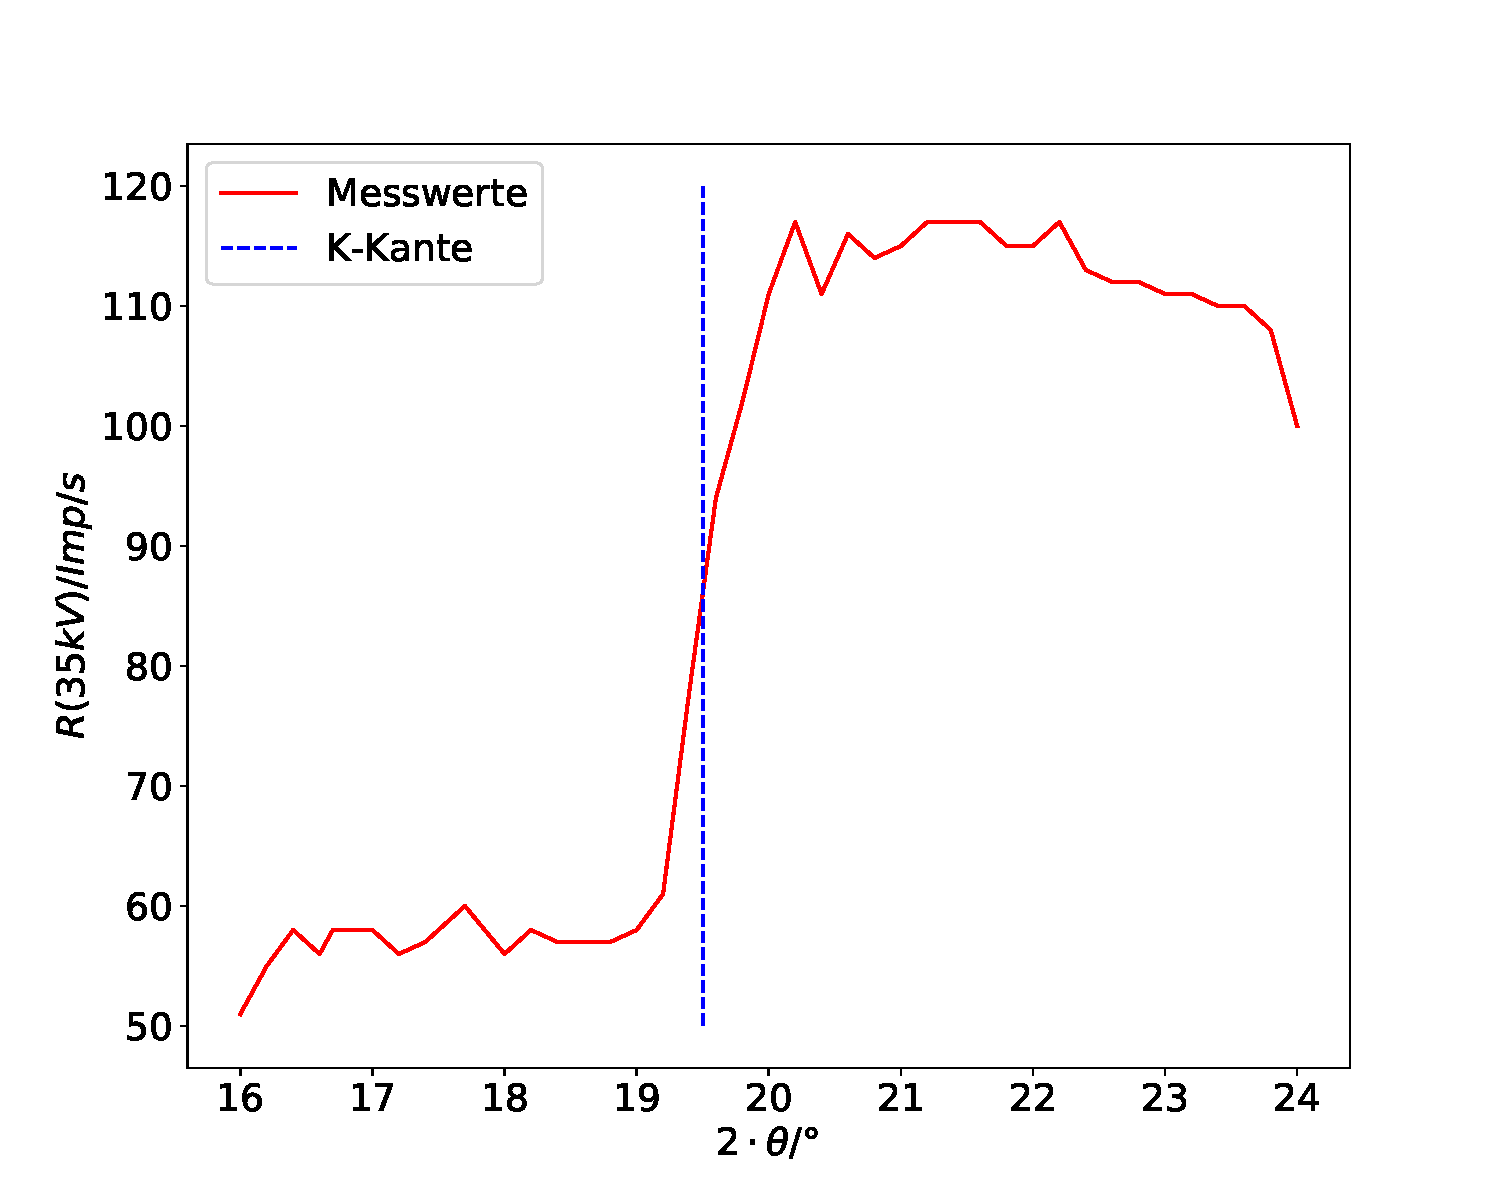
\includegraphics[width=\textwidth]{zirkonium.pdf}
  \caption{Absorptionsspektrum von Zirkonium}
  \label{fig:zirkonium}
\end{figure}

Die Abschirmkonstante $\sigma_K$ berechnet sich mit Hilfe der Formel (\ref{eqn:bindungsenergie}).
Dafür wird der Zusammenhang
\begin{equation*}
  z_{\symup{eff}}= z-\sigma
\end{equation*}
verwendet.
Somit ergibt sich
\begin{equation*}
  \sigma_K = Z - \sqrt{\frac{E}{R_{\infty}}}
\end{equation*}
mit $Z_{Br} = 35$, $Z_{Sr}= 38$ und $Z_{Zr}= 40$ (\cite{Z})
ergeben sich die Abschirmkonstanten zu
\begin{align}
  \sigma_{K_{Br}} &= 3,340\\
  \sigma_{K_{Sr}} &= 3,325\\
  \sigma_{K_{Zr}} &= 3,442
  \label{eqn:sig}
\end{align}

Im folgenen Wird $\sqrt{E}$ gegen Z aufgetragen.
Außerdem wird eine lineare Regression mit
\begin{equation*}
  \sqrt{E} = a\cdot Z +b
\end{equation*}
durchgefürt.
Die bestimmten Parameter lauten
\begin{align*}
  a &= (1,449 \pm 0,026)\cdot 10^{-9}\, \mathrm{\sqrt{J}}\\
  b &= (-3,9\pm 1,0)       \cdot 10^{-9}\, \mathrm{\sqrt{J}}
\end{align*}
Die Regression ist in Abbildung \ref{fig:Z} zu sehen.
\begin{figure}
  \centering
  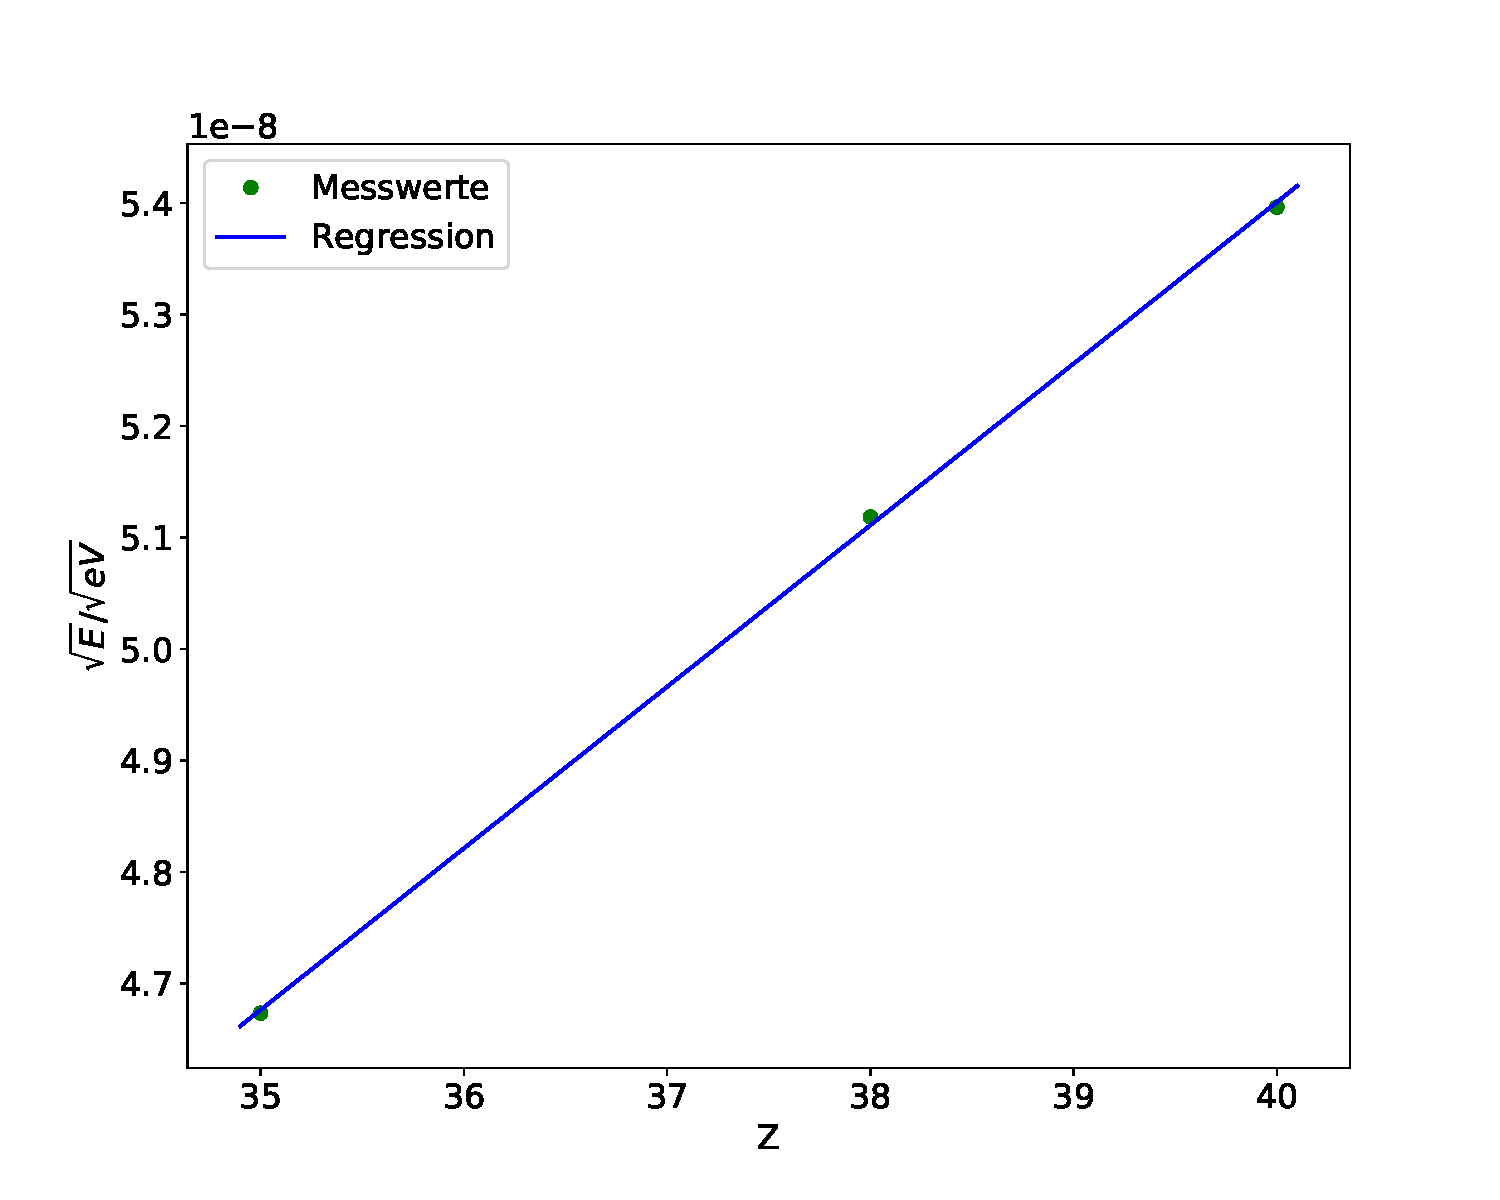
\includegraphics[width=\textwidth]{Z.pdf}
  \caption{lineare Regression}
  \label{fig:Z}
\end{figure}
Aufgrund der Formel (\ref{eqn:bindungsenergie}) ergibt sich die Rydbergkonstante zu
\begin{equation*}
  R_{\infty} = a^2 = (13,105 \pm 0,470)\,\mathrm{eV}
\end{equation*}
Der Fehler berechnet sich mit
\begin{equation*}
  \Delta_{R_{\infty}} = 2a\cdot\Delta a
\end{equation*}
\\
Im Folgenden wird das Absorptionsspektrum von Quecksilber betrachtet.
\begin{align*}
\theta_{L2} = 12,7°\\
  \theta_{L3} = 14,7°
\end{align*}
Daraus ergeben sich mit den Formeln (\ref{eqn:bragg})
und (\ref{eqn:wellenlänge}) die Energien und die Energiedifferenz
\begin{align*}
E_{\theta_{L2}} = 14,00\,\mathrm{keV}\\
E_{\theta_{L3}} = 12,13\,\mathrm{keV}\\
\Delta E = 1,87\,\mathrm{keV}
\end{align*}
Mit Formel (\ref{eqn:sigma}) ergibt sich nun die Abschirmkonstante $\sigma_L$
\begin{equation*}
  \sigma_L = 4,074
\end{equation*}
Die Ordnungszahl von Quecksilber beträgt $Z=80$.
\begin{figure}
  \centering
  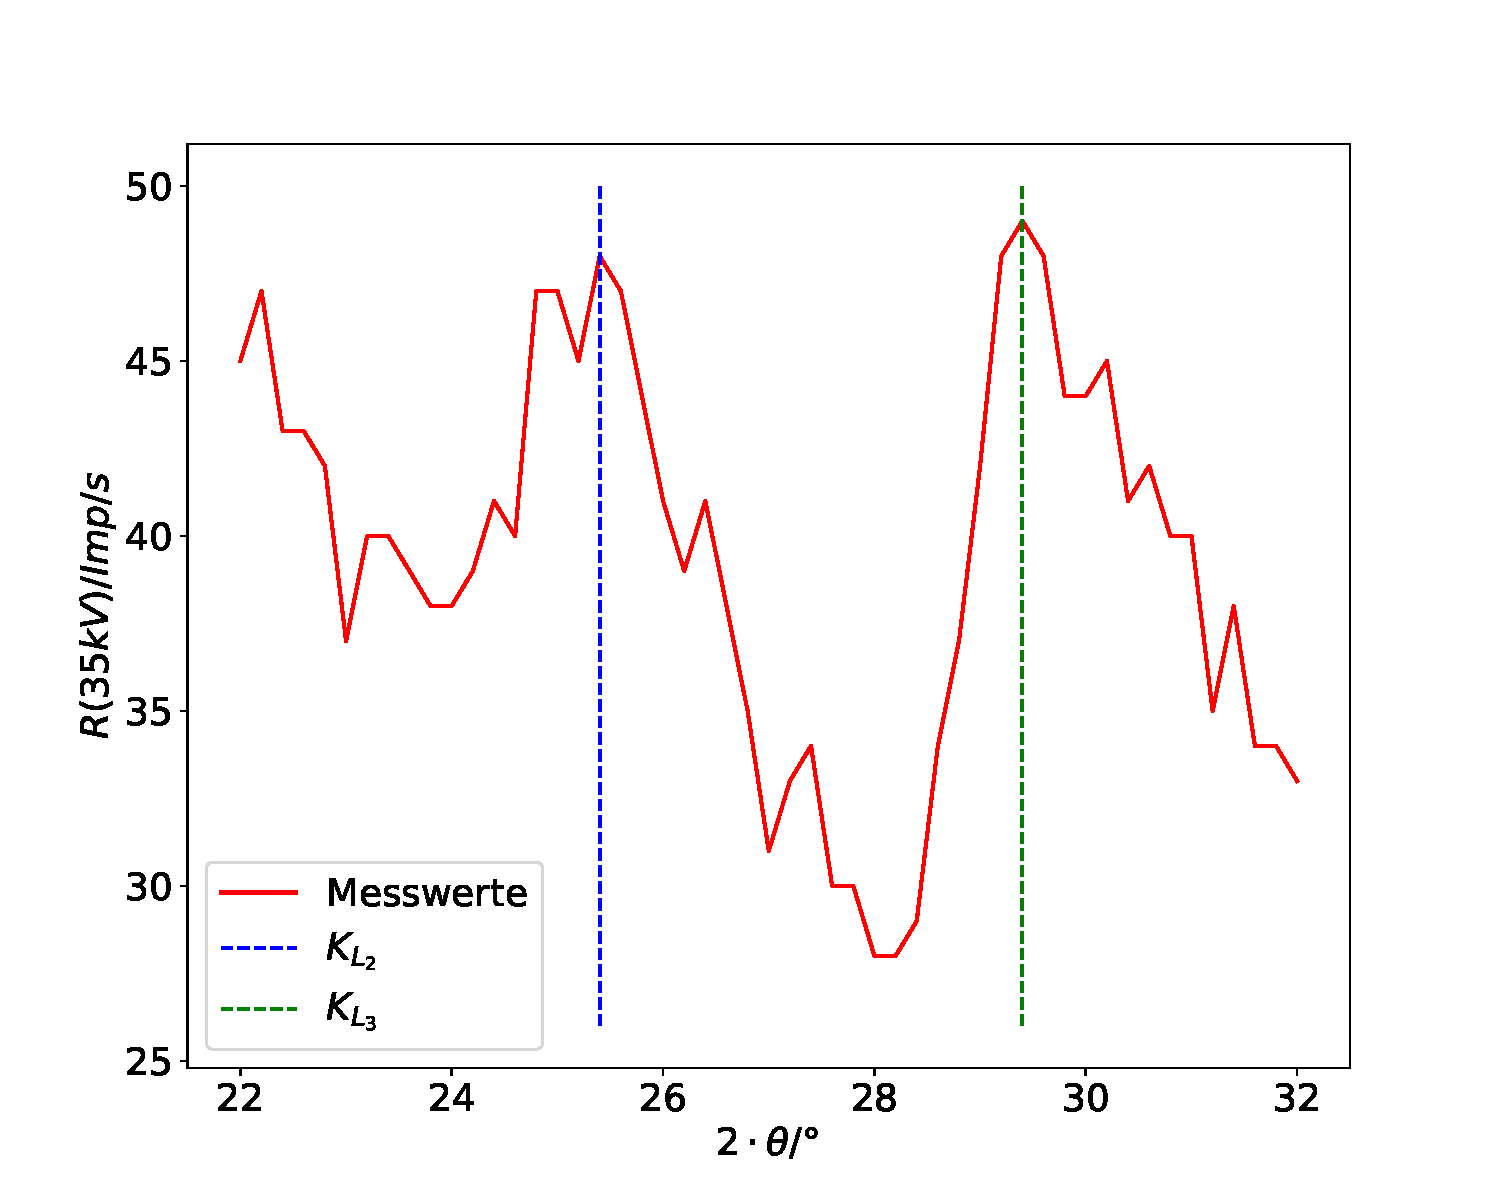
\includegraphics[width=\textwidth]{hg.pdf}
  \caption{Absorptionsspektrum von Quecksilber}
  \label{fig:hg}
\end{figure}

\section{Diskussion}
Im ersten Teil des Versuchs wurde der Sollwinkel bestimmt.
Mit einer bweichung von 1,07\%, weißt dieser keine große Abweichung zum eingestellten Wert auf.
\begin{align*}
  \theta_{eingestellt} &= 14°\\
  \theta_{bestimmt} &= 14,15°
\end{align*}
\\
Im zweiten Teil wurde zunächst die maximale Energie des bremsspektrum bestimmt.
Auch diese weicht mit 0,91\% nur gering von dem zu erwartenden Wert ab.
\begin{align*}
  \theta_{theo} &= 35\,\mathrm{keV}\\
  \theta_{exp} &= 35,317\,\mathrm{keV}
\end{align*}
%Zudem wurde die Abschirmkonstante $\sigma_k$ bestimmt.
%Mit 4,45\% ist die Abweichung zum Theoriewert ebenfalls gering.
%\begin{align*}
%  \sigma_{k,theo} &= 13,03\\
%  \sigma_{k,exp} &= 13,161
%\end{align*}
\\
Im dritten Teil wurden zunächst die Abschirmkonstanten für Brom, Strontium und Zirkonium bestimmt.
Mit den Ergebnissen aus (\ref{eqn:sig}) und den Literaturwerten
\begin{align*}
\sigma_{Brom} &= 3,85\\
\sigma_{Strontium} &= 4\\
  \sigma_{Zirkonium} &= 4,1
\end{align*}
ergeben sich die prozentualen Abweichungen zu:
\begin{align*}
p(Br) &= 13,25\%\\
p(Sr) &= 18,75\%\\
  p(Zr) &= 16,05\%
\end{align*}
Die Abweichung lassen sich auf die Bestimmung der Werte zurückführen.
Die genutzten Werte wurden aus den erhaltenden Plots abgelesen.
Dies führ zu Fehlern.\\
Mit Hilfe einer lienaren Regression wurde nun die Rydbergkonstante bestimmt.
Die Abweichung von 3,64\% lässt sich mit den vorangegangenen Fehlern erklären.
Aufgrund des entstandenen Plots war keine größere Abweichung zu erwarten.\\

Zum Schluss wurde die Abschirmkonstante für Quecksilber bestimmt.
Die Abweichung von 13,80\% wird mithilfe des Literaturwertes bestimmt. \cite{4}

\begin{align*}
\sigma_{L,theo} &= 3,58\\
  \sigma_{L,exp} &= 4,074
\end{align*}
